\documentclass[a4paper, 12pt]{article}
\usepackage[a4paper,top=1.3cm,bottom=2cm,left=1.5cm,right=1.5cm,marginparwidth=0.75cm]{geometry}
\usepackage{wrapfig}
\usepackage{graphicx}
\usepackage{mathtext}
\usepackage{amsmath}
\usepackage{siunitx}
\usepackage{subfigure}
\usepackage{multirow}
\usepackage{rotating}
\usepackage[T1,T2A]{fontenc}
\usepackage[russian]{babel}
\usepackage{caption}

\graphicspath{{pictures/}}
\begin{document}
	\pagenumbering{gobble}
	\pagenumbering{arabic}
	

	\title{\textbf{Определение теплоты испарения жидкости. (2.4.1)}}
	\author{Зайнуллин Амир}
	\maketitle

	\section{Аннотация}
	
	\textbf{Цель работы:} 1) измерение давления насыщенного пара жидкости при разной температуре; 2) вычисление по полученным данным теплоты испарения с помощью уравнения Клапейрона-Клаузиуса. \\
	\textbf{В работе используются:} термостат, герметический сосуд, заполненный водой, отсчётный микроскоп.
	
	
	\section{Теоретические сведения}
	Количество теплоты, необходимое для изотермического испарения одного моля жидкости при внешнем давлении, равном упругости ее насыщенных паров, называется молярной теплотой испарения (парообразования). \\
	В данной работе используется метод, основанный на формуле Клапейрона-Клаузиуса (1).
	
	\subsection*{Уравнение Клапейрона-Клаузиуса}
	\begin{equation}
		\frac{dP}{dT}=\frac{L}{T\left(V_2-V_1\right)}.
	\end{equation}
	Здесь $ P $ -- давление насыщенного пара жидкости при температуре $ T $, $ T $ -- абсолютная температура жидкости и пара, $ L $ -- теплота испарения жидкости, $ V_2 $ -- объем пара, $ V_1 $ -- объем жидкости. Найдя из опыта $ dP/dT $, $ T $, $ V_2 $ и $ V_1 $, можно определить $ L $ путем расчета. Величины $ L $, $ V_2 $ и $ V_1 $ в формуле (1) должны относиться к одному и тому же количеству вещества; мы будем относить их к одному молю.

	Так как удельный объем жидкости мал по сравнению с удельным объемом пара, мы можем им пренебречь. Аналогично можно заметить малость коэффициента $b$ в уравнении Ван-Дер-Ваальса. Значит им можно пренебречь. Пренебрежение членом $\dfrac{a}{V^2}$ вносит ошибку менее 3 процентов. Тогда уравнение Ван-Дер-Ваальса будет как для идеального газа. Выразим объем. \\
	\[ V = \dfrac{RT}{P} \] 
	
	\subsection*{Формула для теплоты испарения жидкости}

	\begin{equation}
		L = \frac{RT^2}{\mu P}\frac{dP}{dT} = - \frac{R}{\mu} \frac{d(ln P)}{d(1/T)}
	\end{equation}
	
	
	Как видим, если измерить зависимость давления насыщенных паров от температуры по формуле (2) можно получить удельную теплоту испарения.
	
	\section{Экспериментальная установка}
	Измерения проводятся на установке, изображенной на рис. 1. С помощью термостата A выставляется желаемая температура, и с помощью микроскопа C измеряется положение менисков ртути в U-образном монометре 15. Давление насыщенных паров считается как разность высот менисков ртути.
	Измерения проводятся в 2 этапа. В начале жидкость нагревается, а потом остужается. Это делается для того, чтобы посмотреть зависит ли давление насыщенных паров только от состояния жидкости или нет.
	
	\begin{figure}[!ht]
		\center{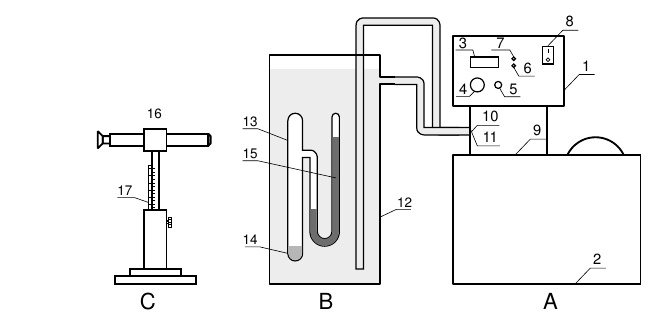
\includegraphics[width=\textwidth]{ustanovka}}
		\caption{Установка для определения давления насыщенных паров.}
	\end{figure}

	\newpage

	\section{Результаты измерений и обработка данных}
	Измеряем давление по вышеописанной схеме. В таблице (1) $h_1$ и $h_2$ это координаты левого и правого менисков соответственно относительно некоторой точки. 
	Для ошибок измерения имеем следующее
	\begin{align*}
		\Delta h &= 0,05 \hspace{2pt} мм\\
		\Delta T &= 0,1 \hspace{2pt} ^\circ C
	\end{align*}
	Используемая формула для давления и его погрешности
	\[ \Delta P = \rho g (h_2 - h_1) \] 
	\[ \sigma_{\Delta P} =  \dfrac{2 \Delta h}{h_2 - h_1} \Delta P\]
	Но, посчитав относительную погрешность измерения разности высот, получим что она не больше 0,5 процентов. Пренебрежем ею.


	\begin{table}[!ht]
		\centering
		\begin{tabular}{|c|c|c|c|c|c|c|c|}
		\hline
			№ & $T, ^\circ C$ & $T$, К & $h_1, мм$ &  $h_2, мм$ & $\Delta P$, Па & $\dfrac{1}{T} \cdot 10^3$, $\dfrac{1}{\text{К}}$ & ln($P$) \\ \hline
			1 & 21 & 294 & 80,2 & 97,2 & 2258 & 3,40 & 7,72 \\ \hline
			2 & 22 & 295 & 81,3 & 97,7 & 2178 & 3,39 & 7,69 \\ \hline
			3 & 23 & 296 & 80,2 & 98,1 & 2378 & 3,38 & 7,77 \\ \hline
			4 & 24 & 297 & 79,4 & 98,8 & 2577 & 3,37 & 7,85 \\ \hline
			5 & 25 & 298 & 79,1 & 99,6 & 2723 & 3,36 & 7,91 \\ \hline
			6 & 26 & 299 & 78,5 & 100,2 & 2882 & 3,34 & 7,97 \\ \hline
			7 & 27 & 300 & 77,4 & 101,3 & 3175 & 3,33 & 8,06 \\ \hline
			8 & 28 & 301 & 76,7 & 102,3 & 3400 & 3,32 & 8,13 \\ \hline
			9 & 29 & 302 & 75,7 & 102,9 & 3613 & 3,31 & 8,19 \\ \hline
			10 & 30 & 303 & 74,7 & 103,9 & 3879 & 3,30 & 8,26 \\ \hline
			11 & 31 & 304 & 74,2 & 105,5 & 4157 & 3,29 & 8,33 \\ \hline
			12 & 32 & 305 & 73,3 & 106,1 & 4357 & 3,28 & 8,38 \\ \hline
			13 & 33 & 306 & 72,4 & 107,1 & 4609 & 3,27 & 8,44 \\ \hline
			14 & 34 & 307 & 71,4 & 108 & 4861 & 3,26 & 8,49 \\ \hline
			15 & 35 & 308 & 70,5 & 109,3 & 5154 & 3,25 & 8,55 \\ \hline
			16 & 36 & 309 & 69,5 & 110,5 & 5446 & 3,24 & 8,60 \\ \hline
			17 & 37 & 310 & 68,6 & 111,3 & 5672 & 3,23 & 8,64 \\ \hline
			18 & 38 & 311 & 67,7 & 112,7 & 5977 & 3,22 & 8,70 \\ \hline
			19 & 39 & 312 & 66,7 & 113,5 & 6216 & 3,21 & 8,73 \\ \hline
			20 & 40 & 313 & 65,7 & 114,9 & 6535 & 3,19 & 8,78 \\ \hline
		\end{tabular}
		\caption{Таблица измерений}
	\end{table}

	\newpage

	\begin{figure}[!ht]
		\centering
		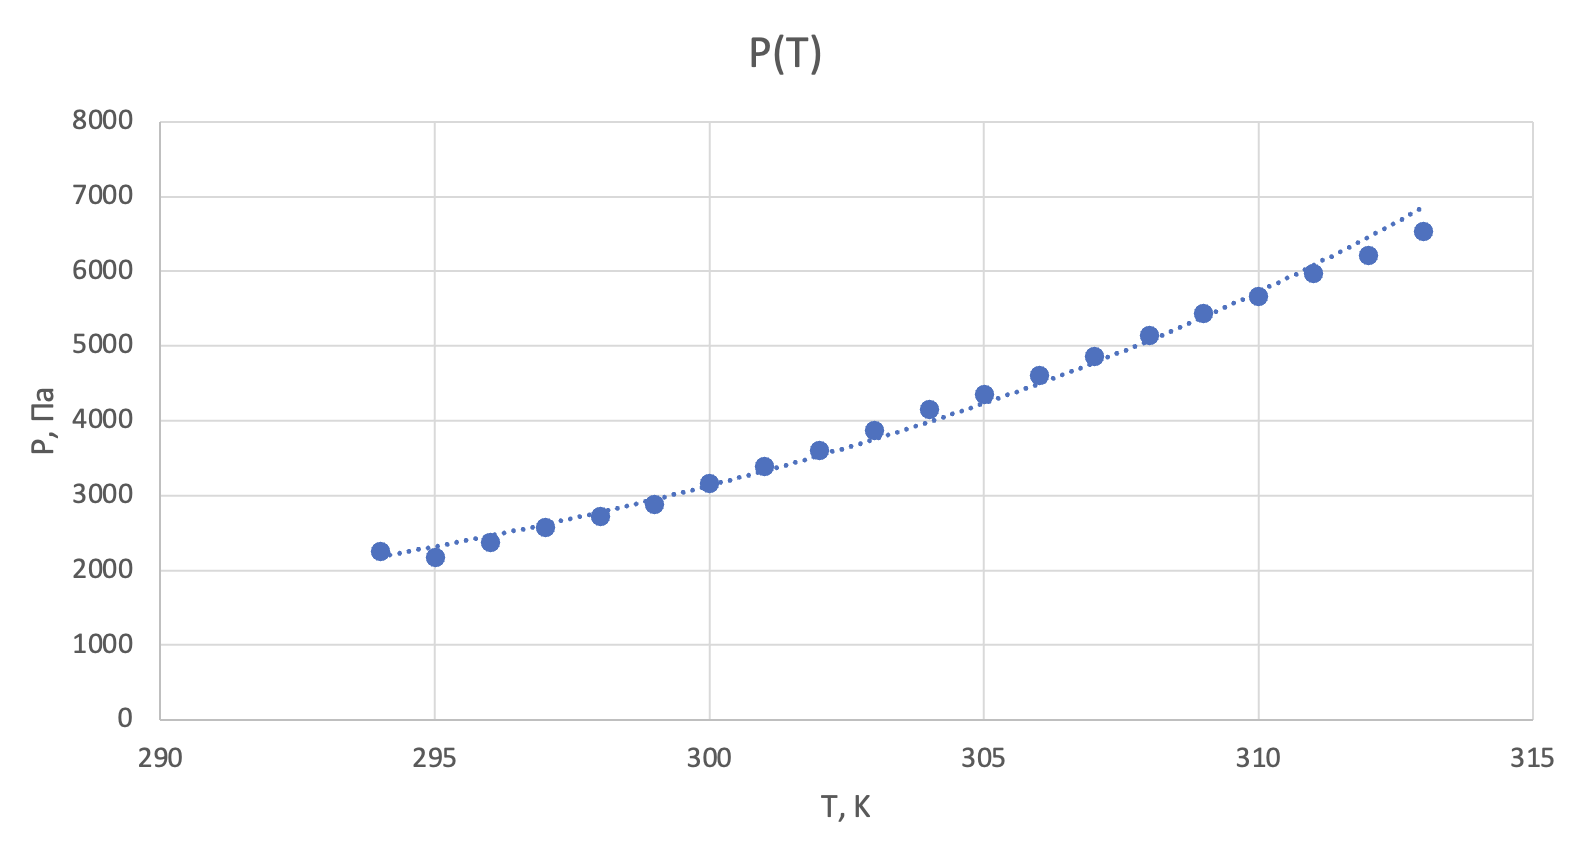
\includegraphics[width=0.8\textwidth]{2.png}
		\caption{Зависимость давления от температуры}
	\end{figure}


	

	\begin{figure}[!ht]
		\centering
		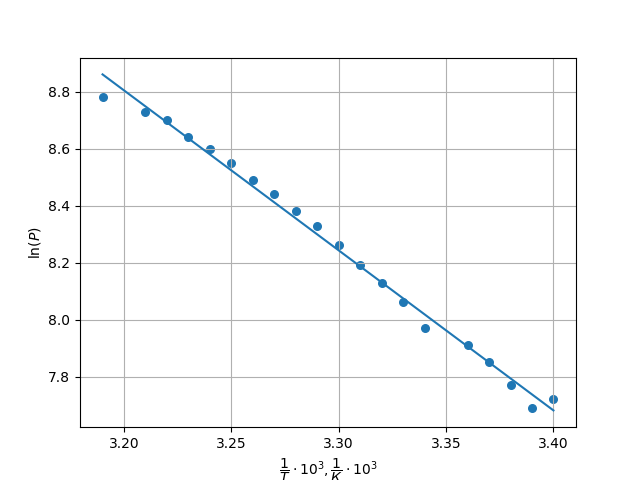
\includegraphics[width=0.8\textwidth]{Figure_1.png}
	\end{figure}

	Посчитаем коэффициент наклона графика по МНК. Полная погрешность коэффициента наклона графика будет состоять только из случайной погрешности, так как системной мы пренебрегли.
	\[ \frac{d(lnP)}{d(1/t)} = \frac{\langle \ln P \cdot \dfrac{1}{T} \rangle - \langle \dfrac{1}{T} \rangle \langle \ln P \rangle}{\langle \dfrac{1}{T^2} \rangle - \langle \dfrac{1}{T} \rangle ^2} \]
	\[ \sigma_{случ} = \frac{1}{\sqrt{n}} \cdot \sqrt{\frac{\langle ln^2 P \rangle - \langle ln P \rangle^2}{\langle \dfrac{1}{T^2} \rangle - \langle \dfrac{1}{T} \rangle ^2} - \frac{d(lnP)}{d(1/t)}} \]
	\[ \frac{d(lnP)}{d(1/t)} = (-5614 \pm 95) \hspace{4pt} К \\ \] 
	По формуле (2) найдем теплоту парообразования.
	\[ L = (2590 \pm 38) \hspace{4pt} кДж/кг\\ \]

	\section{Обсуждение результатов и выводы}

	В данной лабораторной работе мы:
	\begin{enumerate}
		\item Исследовали зависимость давления насыщенных паров воды от давления жидкости
		\item Вычислили теплоту парообразования воды
	\end{enumerate} 
	Сравним полученные данные с табличными. Из справочников $L = 2260$ кДж/кг. Достаточно большое расхождение около десяти процентов может быть вызвано большим количеством причин. Во-первых в нашей модели мы использовали некоторые упрощения в формуле 
	Клапейрона-Клаузиуса. Мы пренебрегли некоторыми членами: удельным объемом воды и слагаемым $b$ в уравнении Ван-Дер-Ваальса. Во-вторых возможно мы не достаточно много ждали когда установится тепловое равновесие. В третьих, теплота парообразования может зависеть от температуры, что мы не учли в опыте. 
	\par Для увеличения точности измерений можно уменьшить диапазон измеряемых температур. Тогда изменением теплоты парообразования можно будет пренебречь, и это внесет меньшую погрешность. 
	\newpage

	

\end{document}

